% -----------------------------------------------------------------------
% CCN Conference - Extended Abstract Track Template
% For papers up to 2 pages (excluding references); no supplement.
% -----------------------------------------------------------------------
\documentclass[submission]{ccn}  % options: submission (default), preprint, extended-abstract
\usepackage{graphicx}
% TODO: For preprints (not accepted), use:
%   \documentclass[preprint]{ccn}

% TODO: For camera-ready extended abstract (after acceptance), use:
%   \documentclass[extended-abstract]{ccn}

% TODO: Add your bibliography file(s).
\addbibresource{ccn_references.bib}


\title{Ecological Data and Temporal Prediction Align DNNs with Human Vision}

% Authors are automatically anonymized in submission mode.
%
% --- STYLE 1: Single author ---
% \author{Jane Smith \\
%   Department of Neuroscience, University Name \\
%   \email{jane@example.edu}}
%
% --- STYLE 2: Multiple authors, same affiliation (comma-separated, no \And) ---
% \author{Jane Smith, John Doe, and Alice Brown \\
%   Department of Neuroscience, University Name \\
%   \email{\{jane,john,alice\}@example.edu}}
%
% --- STYLE 3: Two authors, different affiliations (use \And) ---
% \author{First Author \\
%   Department of Example, University Name \\
%   \email{first@example.edu}
%   \And Second Author \\
%   Another Department, Another University \\
%   \email{second@example.edu}}
%
% --- STYLE 4: Many authors, traditional format (use \AND for row breaks) ---
% \author{Author One \\
%   Dept of Neuroscience, First Univ \\
%   \email{one@first.edu}
%   \And Author Two \\
%   Dept of Psychology, Second Univ \\
%   \email{two@second.edu}
%   \AND Author Three \\   % \AND starts a new row
%   Dept of Biology, Third Univ \\
%   \email{three@third.edu}
%   \And Author Four \\
%   Dept of Physics, Fourth Univ \\
%   \email{four@fourth.edu}}
%
% --- STYLE 5: Many authors, compact format (recommended for 3+ authors) ---
% Use \affmark{} for superscript numbers, \affiliation{} to define them,
% and optionally \emails{} for a shared email line.
\author{%
  Peisen Zhou\affmark{1} \And
  Drew Linsley\affmark{1} \And
  Akash Nagaraj\affmark{1} \And
  Alekh K. Ashok\affmark{1} \AND
  Thomas Serre\affmark{1}%
}
\affiliation{1}{Department of Cognitive and Psychological Sciences, Brown University\\ Providence, RI, USA}
\emails{peisen\_zhou@brown.edu}


\begin{document}
\maketitle
\cleardoublepage


% \section{Abstract}{}
% \begin{quote}
% \small
% \textbf{Keywords:} Computer Vision; Saliency Alignment
% \end{quote}
\section{Abstract}{A long tradition in computational neuroscience proposes that temporal structure in visual experience shapes how biological systems learn to see. Deep neural networks (DNNs), typically trained on static labeled images, lack this inductive pressure. Could the learning regime explain their growing misalignment with human vision? We fine-tuned large pretrained vision transformers on naturalistic video of real-world objects, systematically comparing self-supervised objectives that range from reconstructing the current frame, to interpolating between frames, to predicting the next frame. Next-frame prediction in pixel space produced the largest gain, raising alignment with humans to near the human ceiling while maintaining classification accuracy, with near-human-level viewpoint stability. These results offer a step toward identifying the learning principles that wire up biological vision.}
\begin{quote}
\small
\textbf{Keywords:} Computer Vision; Human Alignment; Self-Supervised Learning; Biological Vision; Predictive Learning
\end{quote}

% \section{Introduction}
% Deep neural networks (DNNs) trained on large-scale image datasets now surpass human performance on a variety of visual tasks. Yet their utility as models of biological vision---for predicting behavior and neural activity---has precipitously declined in recent years \citep{LINSLEY2025}. A key reason is that DNNs and humans rely on different features and strategies when processing visual information\citep{geirhos2022imagenettrainedcnnsbiasedtexture}. Previous work has attempted to close this gap by directly constraining DNN feature importance maps to match human saliency data \citep{fel2022harmonizing}. While effective, this approach sidesteps a fundamental question through supervised learning with human behavioral data: what is the root-cause of DNN misalignment with biological vision? We hypothesize that the divergence between human and DNN visual strategies arises from a more fundamental difference between how they learn about the visual world. If this is the case, then identifying the right learning routine should produce DNNs that achieve human-level accuracy and human-like feature strategies without explicit alignment supervision.
% To test this hypothesis, we trained vision transformers on natural videos of real-world objects rendered from 3D Gaussian Splatting reconstructions using variations of four learning objectives: supervised classification, spatial reconstruction, temporal reconstruction, and temporal prediction. We then evaluated each model's classification accuracy and separately, its alignment with human visual strategies by measuring the correlation between human and model saliency maps and the stability of these maps across viewing angles.
%
% We find that training DNNs to predict future frames in natural video dramatically increases their alignment with human visual strategies, improving saliency map correlation from 0.017 to 0.63 (human ceiling: 0.71), while slightly increasing classification accuracy. Models trained with this objective also exhibit near-human-level representation stability across viewpoints. Notably, these improvements are specific to pixel-level prediction; latent-space variants (i.e., JEPA \citep{assran2023selfsupervisedlearningimagesjointembedding} or DINO-like learning \citep{dinov1}) of the same temporal objectives yield substantially smaller gains. These results suggest that the learning objective is a primary lever for aligning artificial and biological vision, and optimizing over these objectives is a systematic approach towards identifying the principles which wire up biological vision.
\section{Introduction}
Deep neural networks (DNNs) now surpass human performance on many visual tasks, yet their ability to predict human behavior and neural activity has plateaued and in some cases worsened as accuracy has increased \citep{LINSLEY2025}. A key reason is that DNNs and humans rely on different visual features and strategies \citep{geirhos2022imagenettrainedcnnsbiasedtexture}. One response is to directly supervise DNN feature maps with human psychophysics data \citep{fel2022harmonizing}, but this sidesteps a more fundamental question: what learning principles give rise to human-like vision in the first place? A long tradition in computational neuroscience holds that temporal structure in visual experience is central to learning invariant representations. 

F\"{o}ldi\'{a}k's trace rule showed how temporal continuity could teach viewpoint invariance \citep{foldiak1991learning}, and slow feature analysis formalized the broader principle that useful visual features are those that change slowly over time \citep{wiskott2002slow}. Recent work with deep networks supports this view: self-supervised objectives produce ventral-stream-like representations without category labels \citep{zhuang2021unsupervised}, predictive learning over video gives rise to dorsal/ventral specialization \citep{bakhtiari2021functional}, and models trained on egocentric child video develop robust object representations \citep{orhan2024child, lake2017building}. Yet it remains unclear which aspects of temporal learning matter most: the temporal structure itself, the nature of the prediction task, or the space in which learning occurs.

We address this by fine-tuning vision transformers on naturalistic video of real-world objects, systematically varying self-supervised objectives along two axes: temporal task (reconstruct, interpolate, or predict) and target space (pixel or latent). We evaluate each model on classification accuracy and alignment with human visual strategies, measured via human psychophysics and viewpoint stability. We find that next-frame prediction in pixel space produces the largest alignment gain, approaching the human ceiling while maintaining classification accuracy.
\begin{figure*}[ht]
    \begin{center}
        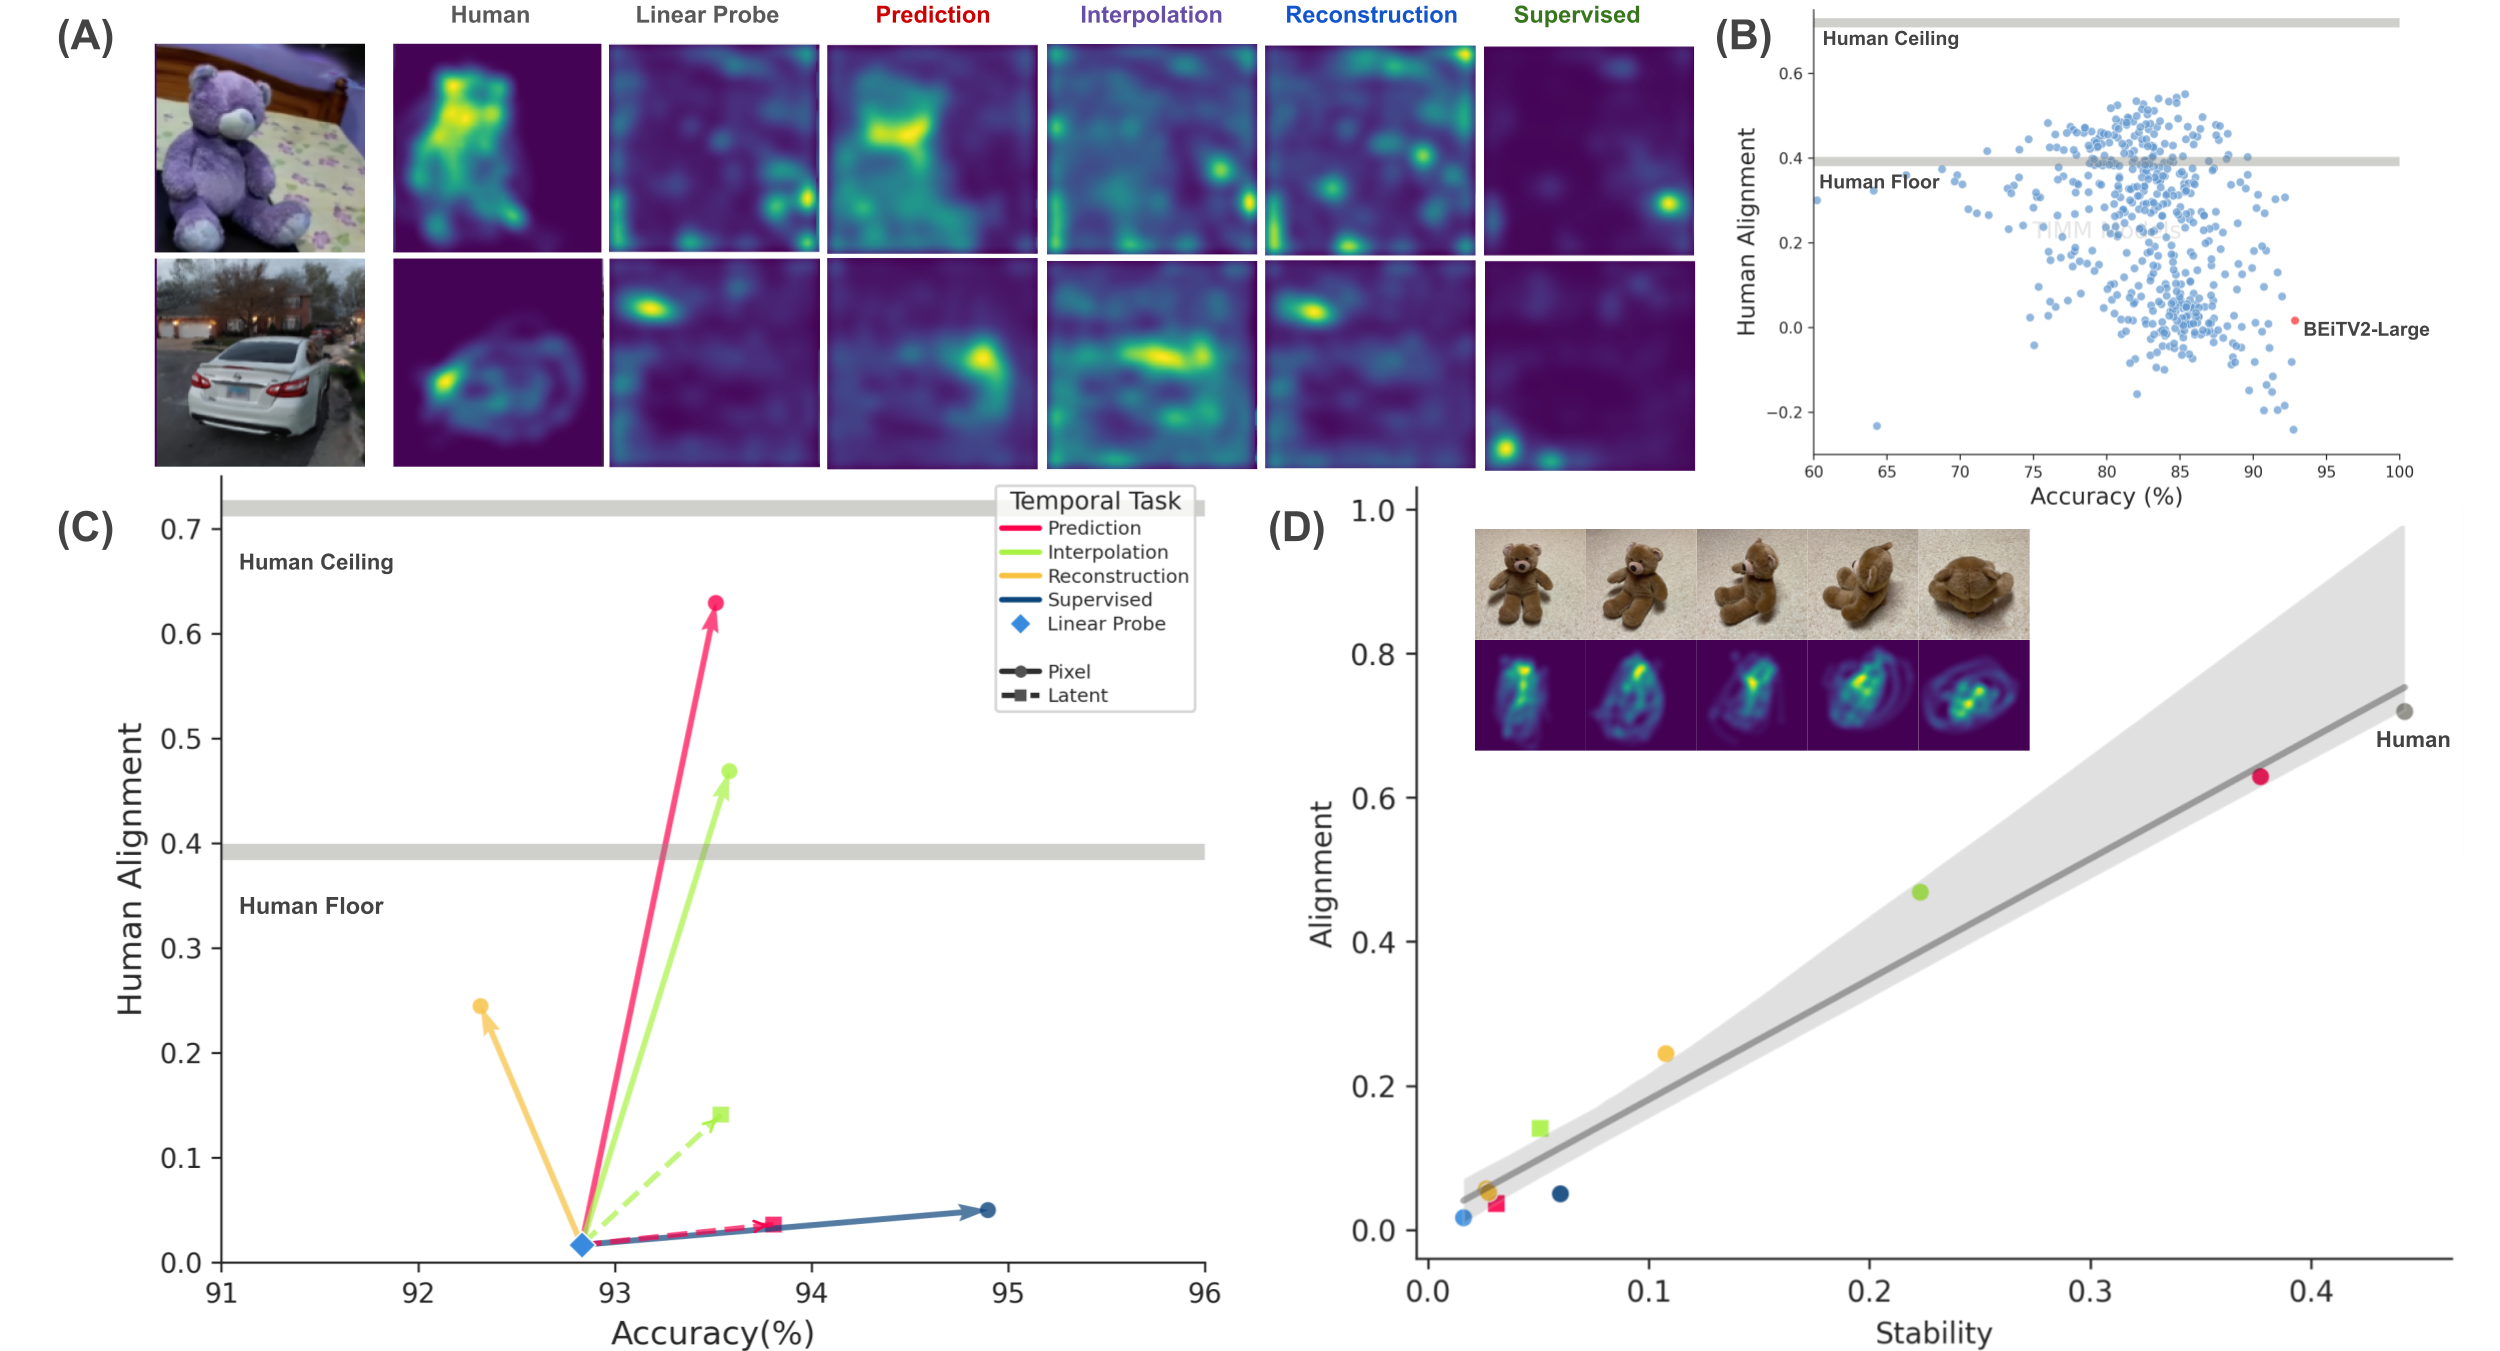
\includegraphics[width=\linewidth]{figures/main.png}
    \end{center}
    \caption{\textbf{Pixel Predict aligns DNNs with human vision.} \textbf{(A)} Feature importance maps from humans and models fine-tuned with different learning objectives. Pixel Predict shifts model importance toward human-like feature strategies. \textbf{(B)} Alignment (correlation between human and model importance maps) vs.\ classification accuracy. Pixel Predict achieves the highest alignment without sacrificing accuracy. Background points show 495 pretrained DNNs from TIMM \citep{rw2019timm}. \textbf{(C)} Representation stability across viewing angles. Pixel Predict produces near-human-level stability. Stability is measured by projecting importance maps across viewpoints using 3D Gaussian Splatting reconstructions and computing correlations at each target angle.}
    \label{fig:result-figure}
\end{figure*}

\section{Approach and Method}

\paragraph{Data generation.}
We used 3D Gaussian Splatting (3DGS) \citep{kerbl3Dgaussians} to generate naturalistic video with two properties not available in standard datasets: smooth, controlled viewpoint trajectories for training, and ground-truth 3D geometry for measuring representation stability across viewing angles. We fit 27,823 3DGS models to Common Objects in 3D (Co3D) \citep{reizenstein21co3d}, which contains videos of real-world objects from 50 MS-COCO categories \citep{mscoco}, and rendered 50 frames along a smooth trajectory per object. Models are trained on sequences of 8 frames sampled at a step size of 4.

Human feature importance maps were collected using ClickMe \citep{linsley2019clickme}, a large-scale online psychophysics platform where participants identify the image regions most relevant to recognizing an object's category. Each importance map is the average across multiple participants.

\paragraph{Model training.} 
To understand how well DNNs align with humans on our dataset, we trained linear probes on 495 DNNs from TIMM \citep{rw2019timm} and measured their classification accuracies and human alignment.
To explore the space of training routines, we fine-tuned an ImageNet-21K \citep{ridnik2021imagenet21kpretrainingmasses} pretrained BEiT-V2 Large \citep{beitv2} from TIMM with seven self-supervised objectives, along with supervised classification as control.
The starting model was selected as a representative SOTA DNN due to its high classification accuracy on our dataset.
% The seven self-supervised objectives are grouped into three categories: spatial reconstruction, temporal reconstruction, and prediction.
% Spatial reconstruction asks models to reconstruct the full or randomly masked parts of images.
% This category includes Masked Autoencoder (MAE) \citep{mae}, VideoMAE \citep{videomae}, and autoencoder \citep{hinton_autoencoder}.
% Temporal reconstruction utilizes temporal information in training videos by asking models to reconstruct intermediate frames of a sequence.
% Finally, the prediction objective makes the models predict the next frame given previous frames as context.
% To maximize the utilization of video information, we implemented temporal reconstruction and prediction using teacher forcing \citep{teacherforcing}.
% Inspired by recent developments in self-supervised learning \citep{dinov1, ijepa}, we included versions of temporal reconstruction and prediction methods with latent-space supervision, using the same design as in \cite{dinov1}.
The seven self-supervised objectives vary along two axes: the temporal task and the target space. The temporal task is one of \textit{reconstruct} (recover the current frame from full or masked input), \textit{interpolate} (fill in intermediate frames in a sequence), or \textit{predict} (generate the next frame from preceding context). Reconstruction includes MAE \citep{mae}, VideoMAE \citep{videomae}, and autoencoder \citep{hinton_autoencoder} variants. For interpolation and prediction, we use teacher forcing \citep{teacherforcing} to leverage the full temporal structure. Each temporal objective is implemented in both pixel space and latent space, the latter following a DINO-style \citep{dinov1} design. 
During self-supervised fine-tuning, we also regularize the model using embeddings from the original pretrained model to prevent catastrophic forgetting of learned visual features.

\paragraph{Alignment evaluation.}
Model feature importance maps are computed by training a linear classification probe on each model and differentiating the output score with respect to the input image.
We then measure human alignment as the Spearman's rank correlation coefficient between the human and model importance maps.

\paragraph{Stability evaluation.} 
We evaluated human and model representation stability by projecting feature importance maps from one angle of an object to other angles, and computing Spearman's rank correlation coefficients between the projected maps and the maps at the target angle.
The projection is achieved using 3D reconstructions from 3D Gaussian Splatting and camera matrices estimated with COLMAP \citep{schoenberger2016sfm, schoenberger2016mvs}.

\section{Results}
% When probed on our datasets, DNNs exhibit a divergence from biological vision similar to that reported in previous research.
% Namely, alignment with humans increases with classification accuracy for weaker models, but decreases with higher accuracy for better-performing models (Fig. 1B).
% Learning routines that utilize temporal information break this trend and yield models with greater human alignment without losing classification accuracy.
% Pixel-level temporal prediction produces the greatest improvement in alignment.
% Specifically, alignment increases from 0.017 to 0.63 (Human Ceiling: 0.71).
% To our surprise, latent versions of temporal learning routines have much smaller effects on alignment.
% When examining the model saliency map, we see that the same routine produces maps that focus on the foreground and features similar to those found in human saliency maps (Fig. 1A).
% Stability
Among 495 pretrained DNNs, alignment with humans increases with classification accuracy for weaker models but decreases for stronger ones (Fig.~\ref{fig:result-figure}B), consistent with prior reports of a divergence between DNN performance and biological plausibility. Self-supervised fine-tuning with temporal objectives breaks this trend. Pixel Predict produces the largest alignment gain, raising correlation between human and model importance maps from 0.017 to 0.63 (human ceiling: 0.71) without loss of classification accuracy. Qualitatively, Pixel Predict importance maps shift toward the foreground features highlighted in human maps (Fig.~\ref{fig:result-figure}A). Latent-space variants of the same temporal objectives yield much smaller improvements, indicating that alignment depends on pixel-level optimization, not just temporal structure. Pixel Predict also produces near-human-level representation stability across viewing angles (Fig.~\ref{fig:result-figure}C), while other objectives degrade more steeply with angular distance.

%\section{Conclusion}


\newpage
\section{Acknowledgments}

\printbibliography

\end{document}
